\documentclass[10pt,a4paper]{article}
\usepackage[utf8]{inputenc}
\usepackage{amsmath}
\usepackage{amsfonts}
\usepackage{amssymb}
\usepackage[]{algorithm2e}
\usepackage{listings}

\usepackage{graphicx}
\DeclareGraphicsExtensions{.pdf,.png,.jpg,.svg}

\usepackage[left=2cm,right=2cm,top=2cm,bottom=2cm]{geometry}

\setlength\parindent{0pt}

\usepackage{polski}
%\usepackage[latin2]{inputenc}

\title{TIRT - wyszukiwanie obiektów na filmie}

%\author{}
\date{}

\begin{document}
\maketitle

\section{Opis projektu}

Projekt ma na celu wykrywanie obiektów na filmie. W zależności od potrzeb mogą to być różnego rodzaju obiekty. Ze względu na to, że program działa bezpośrednio na pikselach obrazu, poza mocą obliczeniową maszyny, nie ma ograniczeń co do złożoności wykrywanych obrazów. 

Przyjęta metoda polega na przeszukaniu każdej klatki filmu pod kątem wykrycia danego obrazu poprzez okno przesuwne. Dla każdego okna wyznaczana jest klasa (w szczególności, klasyfikator może stwierdzić, że nic tam nie ma). Taka para (okno, klasa) staje się kandydatem na wykrycie obiektu. Dopiero kiedy kilka klatek filmu posiada takiego samego kandydata w bliskim położeniu, wówczas kandydat taki zostaje uznany za wykryty obiekt.

\section{Opis algorytmów}

\subsection{Klasyfikator}

Użyta w projekcie metoda klasyfikacji obrazu jest metodą hashowania opisaną w \cite{splh}. Algorytm polega na obliczeniu liniowej kombinacji składowych obrazu dla każdego bitu hashu:

\begin{equation} \label{hash_equation}
H_i(x) = sgn(w_i \cdot x + b_i) / 2 + 0.5
\end{equation}
gdzie:

$x$ jest wektorem złożonym ze składowych obrazu (subpiksele obrazu).

$H_i$ - $i$-ty bit hashu. 

$w_i$ - wektor wag wyznaczane przez algorytm uczący.

$b_i$ - przesunięcie wyznaczone przez algorytm uczący.

Tak wyznaczonych hash obrazu jest kompaktową informacja o zawartości obrazu. Aby wyznaczyć klasę obrazu, należy znaleźć najbliższy (w sensie odległości Hamminga) hash w bazie. Klasa znalezionego obrazu z bazy jest klasą testowanego obrazu. Zestaw wag $w_i$ oraz $b_i$ nazywamy modelem.

\subsubsection{Uczenie}

Najważniejszym elementem algorytmu hashowania jest uczenie, i.e. wyznaczenie $w_i$ i $b_i$. Metoda opiera się na analizie głównych składowych (ang. Principal Component Analysis, PCA). Wyznaczana jest macierz kowariancji z obrazów ze zbioru uczącego. Wektory własne o największych wartościach własnych stają się wektorami wag $w_i$. Przy czym nie muszą to być wektory własne w sensie formalnym, e.g. nie muszą być ortogonalne. Wersja nadzorowana wykorzystuje także zmodyfikowaną macierz kowariancji, która uwzględnia wiedzę o zaklasyfikowanych przykładach ze zbioru uczącego.

\subsubsection{Specyfikacja}

Algorytm uczący został zaimplementowany w języku c++ w środowisku Visual Studio Express 2013 z użyciem biblioteki Eigen. Składa się z dwóch aplikacji:
\begin{itemize}
  \item SPLH - generująca model
  \item MakeHash - generująca bazę hashy
\end{itemize}

Obrazy są rozmiaru $32 x 32$ RGB, reprezentowane w postaci wektora. Kolejność wartości jest następująca: najpierw wyłącznie składowe czerwone, wiersz po wierszu, następnie składowe zielone, na koniec niebieskie:

\begin{equation} \label{image_pattern}
x = \left[
	\begin{array}{c}
		r_{0,0},
		r_{1,0},
		\cdots,
		r_{31,0},
		r_{0,1},
		\cdots,
		r_{31,31},
		g_{0,0},
		\cdots,
		g_{31,31},
		b_{0,0},
		\cdots,
		b_{31,31},
	\end{array}
\right]
\end{equation}

gdzie $r_{x,y}$ to składowa czerwona o współrzędnych $x$ - nr kolumny i $y$ - nr wiersza. Wartości są z przedziału $(0,1)$. Wagi mają $w_i$ mają taki sam układ jak dane $x$.

Pliki ze zbiorami uczącymi są plikami binarnymi o następującej budowie: Ciąg par $(klasa, obraz)$, przy czym klasa jest liczbą 1 bajtową (255 - oznacza brak klasy), a obraz wektorem $32 \cdot 32 \cdot 3 = 3 072$ bajtów (pojedyncza składowa jest 1 bajtowa) w układzie jak w \ref{image_pattern}.

\

Plik z modelem (class.txt) - plik tekstowy o następującej postaci:

N K

$b_0$ $w_0^{(1)}$ $w_0^{(2)}$ ... $w_0^{(K)}$

$b_1$ $w_1^{(1)}$ $w_1^{(2)}$ ... $w_1^{(K)}$

...

$b_N$ $w_N^{(1)}$ $w_N^{(2)}$ ... $w_N^{(K)}$

Oznaczenia $b_i$ oraz $w_i$ zdefiniowano powyżej.

\

Plik z bazą (\texttt{img\_base.txt}) - plik tekstowy o następującej postaci:

$c_0$ $H_0(x_0)$ $H_1(x_0)$ ... $H_N(x_0)$

$c_1$ $H_0(x_1)$ $H_1(x_1)$ ... $H_N(x_1)$

...

gdzie $c_i$ jest klasą $i$-tego obrazu, a $H_k(x_i)$ jest $k$-tym bitem $i$-tego obrazu.

\subsubsection{Użycie}

Generowanie modelu (wag):

\begin{lstlisting}
SPLH.exe data_bach1.bin data_batch2.bin > class.txt
\end{lstlisting}

Generowanie bazy hashy:

\begin{lstlisting}
MakeHash.exe class.txt data_bach1.bin data_batch2.bin > img_base.txt
\end{lstlisting}

\subsection{Fast hash search}

Sprawne wyszukiwanie hashy w bazie wymaga szybszego algorytmu niż liniowe przeszukiwanie. W projekcie zastosowano algorytm zaprezentowany w \cite{fastHash}. Idea jest naprawdę prosta. $N$ bitowy hash jest dzielony na $K$ równych fragmentów o rozmiarze $N/K$. Jeśli chcemy wyszukiwać hashe odległe o co najwyżej $D$, wówczas dla każdego z K fragmentów realizowanej jest wyszukiwanie sąsiadów odległych o co najwyżej $D/K$. Są to kandydaci na poszukiwane hashe.

\subsubsection{Implementacja}

Przykładowo dla $N=64$, $K=4$, oraz $D=4$, mamy fragmenty wielkości $16$. Daje to $65 536$ możliwych fragmentów. Tak mała liczba umożliwia przygotowanie listy odpowiadających hashy dla każdego możliwego fragmentu. Wyszukanie kandydatów $i$-tego fragmentu sprowadza się sprawdzenia $17$ wcześniej przygotowanych list hashy.

Kiedy w bazie znajdowało się ok. 50 000 hashy, liczba przeszukiwanych hashy dla wyżej podanej konfiguracji wynosiła ok. 100.

\section{Architektura aplikacji}

Właściwa aplikacja wykrywająca składa się z modułów:
\begin{itemize}
  \item Klasyfikacja
  \item Weryfikacja
  \item Rysowanie
\end{itemize}

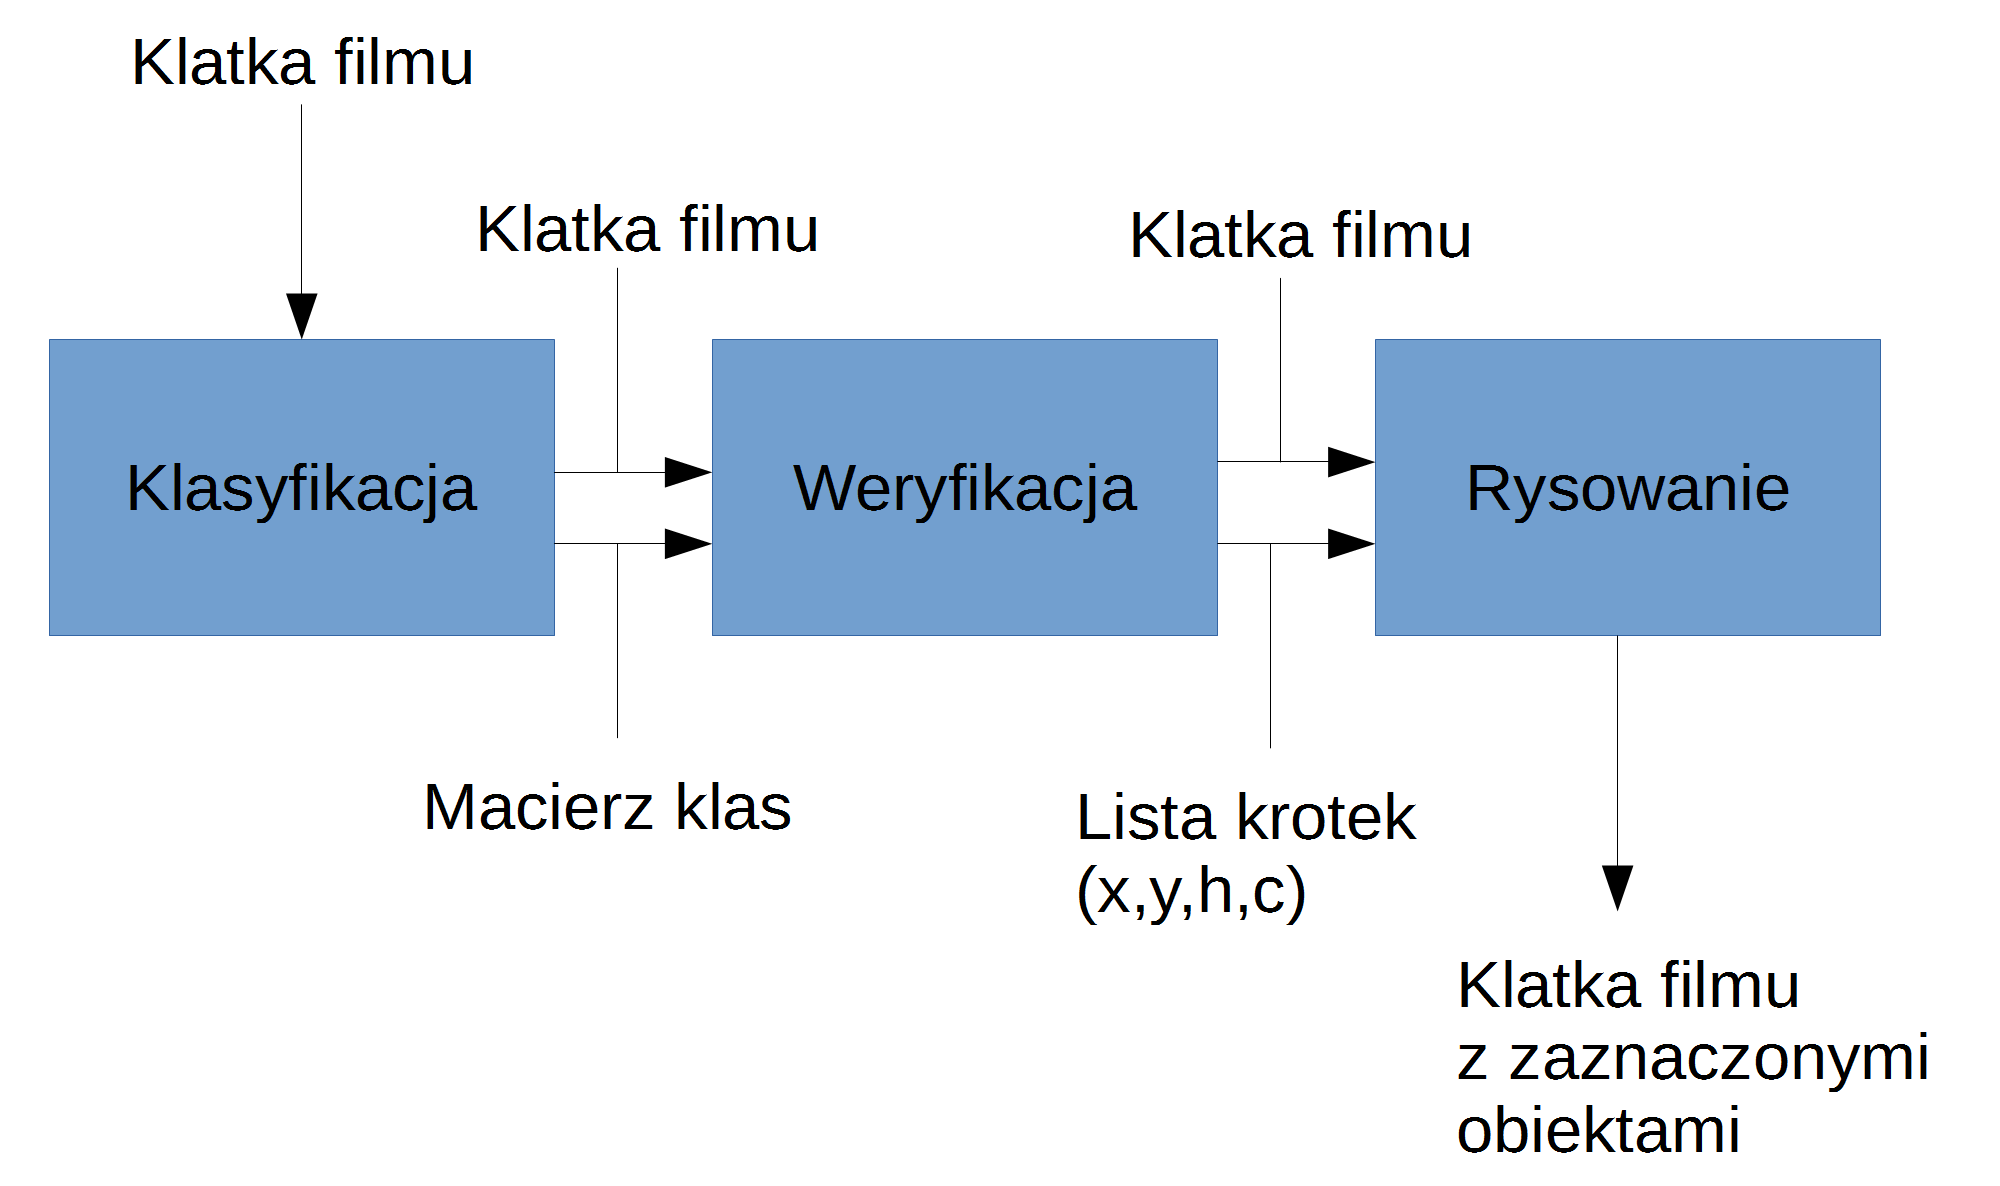
\includegraphics[scale=0.3]{diagram.png}

\subsection{Klasyfikacja(classifier.py)}

Moduł klasyfikujący buduje macierz klas kandydatów. Wejściem są kolejne klatki filmu. Tutaj realizowane jest okno przesuwne. Zachowanie się okna definiowane jest przez konfiguracją. Dla każdego położenia okna wycinany jest obraz w nim zawarty, który następnie jest skalowany do rozmiaru klasyfikatora. W tym momencie obraz jest trójwymiarową tablicą liczb z zakresu (0-255). Ze względu na problemy z odczytem takiej tablicy w module klasyfikującym należy tablicę spłaszczyć do jednego wymiaru.

Konfiguracja okna przesuwnego znajduje się w pliku (config.json). Znaczenie elementów konfiguracji:

$horizontal\_density$ - liczba położeń okna w poziomie

$vertical\_density$ - liczba położeń okna w pionie

$size$ - wielkość okna

$classifier\_size$ - wielkość klasyfikatora 

$classes$ - tablica kolorów (w systemie BGR) przypisanych kolejnym klasom.

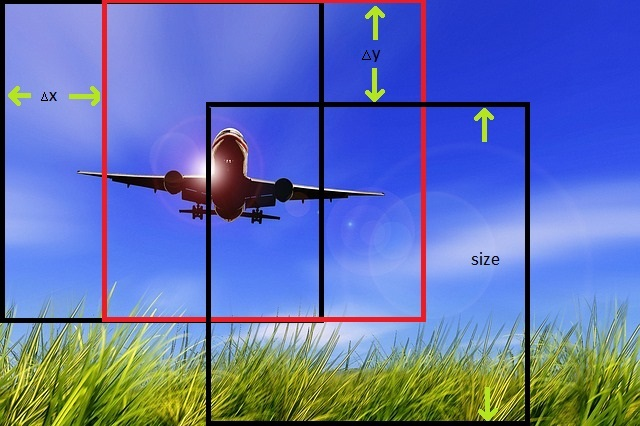
\includegraphics[scale=0.8]{lot.jpg}

Przesunięcie ramki wyniki z następujących wzorów:

$\Delta x = (frame\_width- size)/(horizontal\_density-1)$

$\Delta y = (frame\_height - size)/(vertical\_density-1)$

Wygenerowana macierz jest postaci:

$m_{i,j}$ - klasa obrazu w $i$-tym przesunięci pionowym i $j$-tym przesunięciu poziomym. W przypadku braku klasy wartość $-1$.

Moduł wysyła dalej klatkę filmu i macierz klas.

\subsection{Weryfikacja(verifier.py)}

Moduł weryfikujący bada kilka następujących klatek w celu potwierdzenia poprawności klasyfikacji kandydatów. Aktualna implementacja porównuje każdą klatkę z następną i poprzednią. Dla każdego elementu macierzy klas poszukiwana jest taka sama klasa w macierzy klas poprzedniej i następnej klatki w odległości (w metryce maksimum) co najwyżej 1.

Moduł generuje listę wykrytych obiektów w postaci krotki: $(x, y, h, c)$,
gdzie:

$x$ i $y$ - współrzędne lewego górnego rogu kwadratu w którym znajduje się wykryty obiekt

$h$ - wielkość kwadratu w którym został wykryty obiekt

$c$ - klasa wykrytego obiektu

Dalej wysyłane są klatka filmu i lista obiektów.

\subsection{Rysowanie (picasso.py)}

Moduł rysujący rysuje kwadraty obejmujące wykryte obiekty. Otrzymuje klatkę filmu oraz listę obiektów opisaną w Weryfikacji. Dorysowuje na otrzymanej klatce obramowanie wykrytych obiektów oraz wysyła dalej zmodyfikowaną klatkę. Kolory obramowania pochodzą z konfiguracji (config.json).

\section{Dalszy rozwój}

\subsection{Klasyfikator}
Wykorzystany klasyfikator jest klasyfikatorem typu jednowarstwowa sieć neuronowa, przez co może mieć problemy z rozpoznawaniem bardzie złożonych obiektów. Dobrym pomysłem może być wykorzystanie klasyfikatora wielowarstwowego (e.g. typu autoencoder). Pomysł polega na rekurencyjnym uczeniu zaimplementowanym już algorytmem na danych przetworzonych przez poprzedni przebieg. Przedstawiają to następujące kroki:

Dane 1 - dane uczące jak obecnie

Warstwa 1 - uczenie jak obecnie

Dane 2 - dane 1 przetworzone przez warstwę 1

Warstwa 2 - uczenie jak obecnie, ale na danych 2

Dane 3 - dane 2 przetworzone przez warstwę 2

Warstwa 3 - uczenie jak obecnie, ale na danych 3

... itd. Przy czym każda kolejna warstwa powinna mieć coraz mniej elementów.
 

\subsection{Statystyki}
Ze względu na zdecydowanie zbyt małą spójność wykrytych obiektów postanowiono odłożyć moduł odpowiedzialny za generowanie statystyk na przyszłość. Kiedy osiągnięta zostanie lepsza jakość wykrycia, będzie to z pewnością przydatny moduł. Aby zrealizować ten pomysł wystarczy przesyłać listę wykrytych obiektów w module weryfikującym do nowego modułu statystyki, który zapisywałby w postaci pliku strukturalnego (e.g. xml) informacje o obiekcie (typ, położenie, wielkość).

\subsection{Rozmiar okna}
Ze względu na niewystarczającą wydajność projekt został uproszczony tak, aby wykorzystywana była jedna wielkość okna przesuwnego. Nie jest to znaczącym ograniczeniem możliwości systemu, ponieważ można uruchomić kilka instancji systemu, każdy dla innej wielkości okna przesuwnego. Daje to automatycznie większą możliwość rozproszenia oraz lepiej wykorzystuje maszyny wieloprocesorowe/wielordzeniowe.

\begin{thebibliography}{9}

\bibitem{splh}
  Jun Wang, Sanjiv Kumar, and Shih-Fu Chang,
  Semi-Supervised Hashing for Large Scale Search.
  
\bibitem{fastHash}
  Mohammad Norouzi, Ali Punjani, David J. Fleet,
  Fast Search in Hamming Space with Multi-Index Hashing,
  Department of Computer Science, University of Toronto.

\end{thebibliography}

\end{document}